\documentclass[
  bibliography=totoc,     % Literatur im Inhaltsverzeichnis
  captions=tableheading,  % Tabellenüberschriften
  titlepage=firstiscover, % Titelseite ist Deckblatt
]{scrartcl}

% Paket float verbessern
\usepackage{scrhack}

% Warnung, falls nochmal kompiliert werden muss
\usepackage[aux]{rerunfilecheck}

% unverzichtbare Mathe-Befehle
\usepackage{amsmath}
% viele Mathe-Symbole
\usepackage{amssymb}
% Erweiterungen für amsmath
\usepackage{mathtools}

% Fonteinstellungen
\usepackage{fontspec}
% Latin Modern Fonts werden automatisch geladen
% Alternativ zum Beispiel:
%\setromanfont{Libertinus Serif}
%\setsansfont{Libertinus Sans}
%\setmonofont{Libertinus Mono}

% Wenn man andere Schriftarten gesetzt hat,
% sollte man das Seiten-Layout neu berechnen lassen
\recalctypearea{}

% deutsche Spracheinstellungen
\usepackage[ngerman]{babel}


\usepackage[
  math-style=ISO,    % ┐
  bold-style=ISO,    % │
  sans-style=italic, % │ ISO-Standard folgen
  nabla=upright,     % │
  partial=upright,   % │
  mathrm=sym,        % ┘
  warnings-off={           % ┐
    mathtools-colon,       % │ unnötige Warnungen ausschalten
    mathtools-overbracket, % │
  },                       % ┘
]{unicode-math}

% traditionelle Fonts für Mathematik
\setmathfont{Latin Modern Math}
% Alternativ zum Beispiel:
%\setmathfont{Libertinus Math}

\setmathfont{XITS Math}[range={scr, bfscr}]
\setmathfont{XITS Math}[range={cal, bfcal}, StylisticSet=1]

% Zahlen und Einheiten
\usepackage[
  locale=DE,                   % deutsche Einstellungen
  separate-uncertainty=true,   % immer Unsicherheit mit \pm
  per-mode=symbol-or-fraction, % / in inline math, fraction in display math
]{siunitx}

% chemische Formeln
\usepackage[
  version=4,
  math-greek=default, % ┐ mit unicode-math zusammenarbeiten
  text-greek=default, % ┘
]{mhchem}

% richtige Anführungszeichen
\usepackage[autostyle]{csquotes}

% schöne Brüche im Text
\usepackage{xfrac}

% Standardplatzierung für Floats einstellen
\usepackage{float}
\floatplacement{figure}{htbp}
\floatplacement{table}{htbp}

% Floats innerhalb einer Section halten
\usepackage[
  section, % Floats innerhalb der Section halten
  below,   % unterhalb der Section aber auf der selben Seite ist ok
]{placeins}

% Seite drehen für breite Tabellen: landscape Umgebung
\usepackage{pdflscape}

% Captions schöner machen.
\usepackage[
  labelfont=bf,        % Tabelle x: Abbildung y: ist jetzt fett
  font=small,          % Schrift etwas kleiner als Dokument
  width=0.9\textwidth, % maximale Breite einer Caption schmaler
]{caption}
% subfigure, subtable, subref
\usepackage{subcaption}

% Grafiken können eingebunden werden
\usepackage{graphicx}

% schöne Tabellen
\usepackage{tabularray}
\UseTblrLibrary{booktabs, siunitx}

% Verbesserungen am Schriftbild
\usepackage{microtype}

% Literaturverzeichnis
\usepackage[
  backend=biber,
]{biblatex}
% Quellendatenbank
\addbibresource{lit.bib}
\addbibresource{programme.bib}

% Hyperlinks im Dokument
\usepackage[
  german,
  unicode,        % Unicode in PDF-Attributen erlauben
  pdfusetitle,    % Titel, Autoren und Datum als PDF-Attribute
  pdfcreator={},  % ┐ PDF-Attribute säubern
  pdfproducer={}, % ┘
]{hyperref}
% erweiterte Bookmarks im PDF
\usepackage{bookmark}

% Trennung von Wörtern mit Strichen
\usepackage[shortcuts]{extdash}

\author{%
  Vincent Wirsdörfer\\%
  \href{mailto:vincent.wirsdoerfer@udo.edu}{authorA@udo.edu}%
  \and%
  Joris Daus\\%
  \href{mailto:joris.daus@udo.edu}{authorB@udo.edu}%
}
\publishers{TU Dortmund – Fakultät Physik}


\begin{document}
\section{Diskussion}
\label{sec:Diskussion}

Das Michelson Interferometer arbeitet über Lichtempfindlichkeit, da der Zähler Lichtveränderungen detektiert. 
Außerdem gibt es keine lichtundurchlässige Abschirmung zum Experiment. Dies führt dazu, dass Lichtänderungen 
der Außenwelt das Experiment beeinflussen kann. Gibt es beispielsweise einen Lichtimpuls durch Spiegelungen 
oder eine sich öffnende Tür, so kann der Zähler ein falsch positives Ergebnis zählen. 
Die Lichtveränderungen, welche detektiert werden besitzen eine kleine räumliche Ausdehnung. Aus diesem Grund 
können kleine räumliche Änderungen der Apparatur falsch positive Zählungen zur Folge haben. Beispielsweise 
führen kleine Stöße am Tisch oder dem Messaufbau zu falsch positiven Zählungen. Ein Schlag auf den Tisch kann 
so zu zehn bis 20 Zählungen zu viel führen. Um den Zähler auf die Umgebungshelligkeit zu justieren und so 
falsch positive Ergebnisse zu minimieren, wird der Vorverstärker per Hand kalibriert. Es gibt keine genauen 
Werte dafür und der Drehknopf wird nach Gefühl eingestellt. So kann es sein, dass er zu empfindlich ist, 
was zu erhöhten Werten führt, oder er zu unempfindlich ist, was zu kleinen Werte zur Folge hat. 
Der Motor ist über einen Keilriemen mit der Messschraube verbunden. Der Keilriemen ist allerdings nicht ideal 
gespannt, weshalb Schlupf zwischen Keilriemen und Zahnrad existiert. Aus diesem Grund wird die Mikrometerschraube 
nicht gleichmäßig verstellt und zu schnelle Intensitätswechsel werden ggf. nicht gezählt. Die Skala der 
Messschraube ist leicht verschoben, was ein genaues Ablesen erschwert. Die Zählung wird per Hand gestartet, 
wenn die Mikrometerschraube \qty{2}{\milli \meter} beziehungsweise \qty{5}{\milli \meter} anzeigt und per Hand 
gestoppt, wenn \qty{5}{\milli \meter} verstrichen sind. Dies schließt einen menschlichen Fehler durch nicht 
ideale Reaktionszeiten mit ein.\\

\noindent Als Referenzwert wird die Wellenlänge genommen, welche auf dem Laser steht. Diese beträgt 
$\lambda_\text{Lit} = \qty{635}{\nano \meter}$. Berechnet wurde eine Wellenlänge von 
$\lambda_\text{Lit} = \qty{666\pm6}{\nano \meter}$. Dies ist eine Abweichung von \qty{5\pm0.9}{\percent}.
Grund dafür können die bereits erwähnten Schwierigkeiten bei der Durchführung sein.\\

\noindent Die Luft in der Gaszelle wird mithilfe einer Handpumpe heraus gepumpt, bis ein Unterruck von etwa 
\qty{500}{\milli \meter Hg} entsteht. Dabei ist das Entlüften allerdings nicht gleichmäßig, da die Handpumpe 
schwergängig ist und nach einem Pumpzug der Hebel der Pumpe wieder in Ausgangsstellung gebracht werden muss. 
Dies führt dazu, dass sich der Phasenunterschied der Welle schlagartig ändern kann. Die Photodiode kann daher 
falsch negative Ergebnisse liefern, da die Wechsel der Maxima zu schnell sein können. 
Desweiteren wird nicht immer exakt der gleiche Unterdruck erreicht, was statistische Fluktuationen der Zählrate 
zur Folge hat. Das Belüften der Gaszelle funktioniert gut, da die Lufteinlasschraube gut verstellbar ist. Die 
Luftzufuhr kann so gut gesteuert werden. Die Belüftungszählraten sind so gesehen aussagekräftiger als die 
Entlüftungszählraten.
Nichtsdestotrotz ist der gemessene Brechungsindex von Luft sehr nah an dem Literaturwert. Gerundet auf die gleiche 
Anzahl an signifikanten stellen, stimmen die Werte sogar überein! Die Abweichung beträgt dementsprechend 
\qty{0\pm0.002}{\percent}!\\

Abschließend kann gesagt werden, dass das Experiment trotz einiger technischen Schwierigkeiten sehr genaue 
Werte liefert. Es kann also als gelungen angesehen werden.

%Luftdruck per hand runtergepumpt -> nicht immer exakt gleicher Wert, Wert nicht gleichmäßig herunter gepumpt -> maxima skip


%Umwelteinflüsse in Form von Lichtänderungen und Stößen verfälschen Ergebnis
%Keine gleichmäßige Bewegung der Messschraube aufgrund von unflüssiger Bewegung des Keilriemen
%Skala der Schraube ist aufgrund von Abnutzung leicht verschoben
%Der Selektivverstärker und Schmitt-Trigger wird manuell eingestellt ohne harte Faktoren zu kennen
%Schlupf zwischen Keilriemen und Zahnrad

\section{Anhang}

\begin{figure}
    \centering
    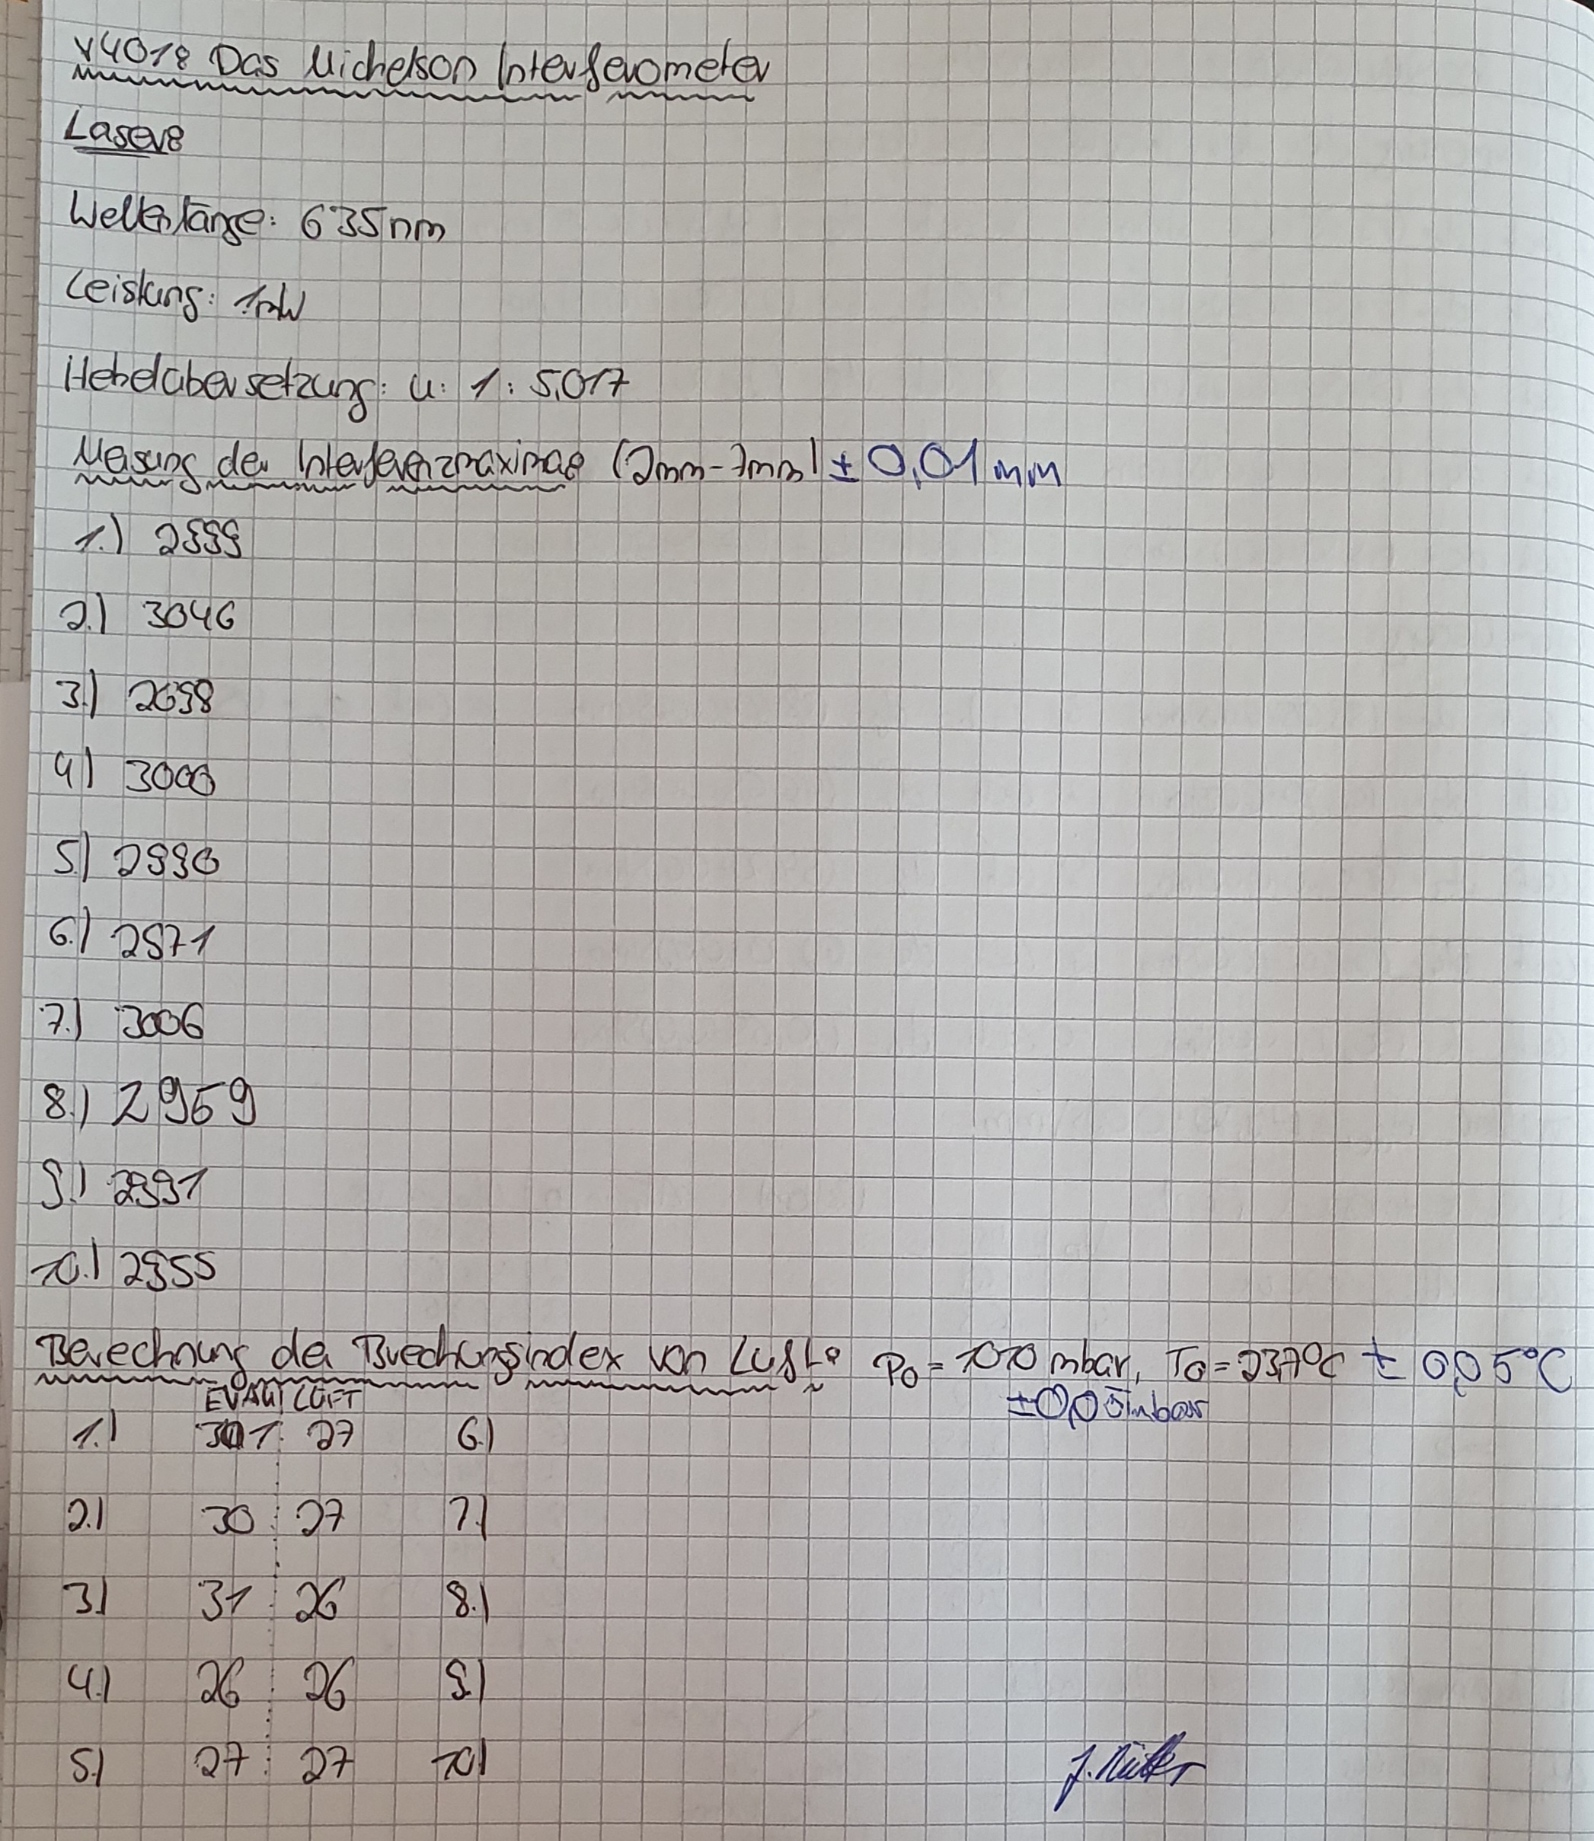
\includegraphics[width=0.9\textwidth]{Laborbuch.jpg}
    \caption{Messdaten im Laborbuch.}
\end{figure}


\end{document}
